\documentclass{standalone}
\usepackage{tikz}
\usetikzlibrary{patterns, positioning}

\begin{document}
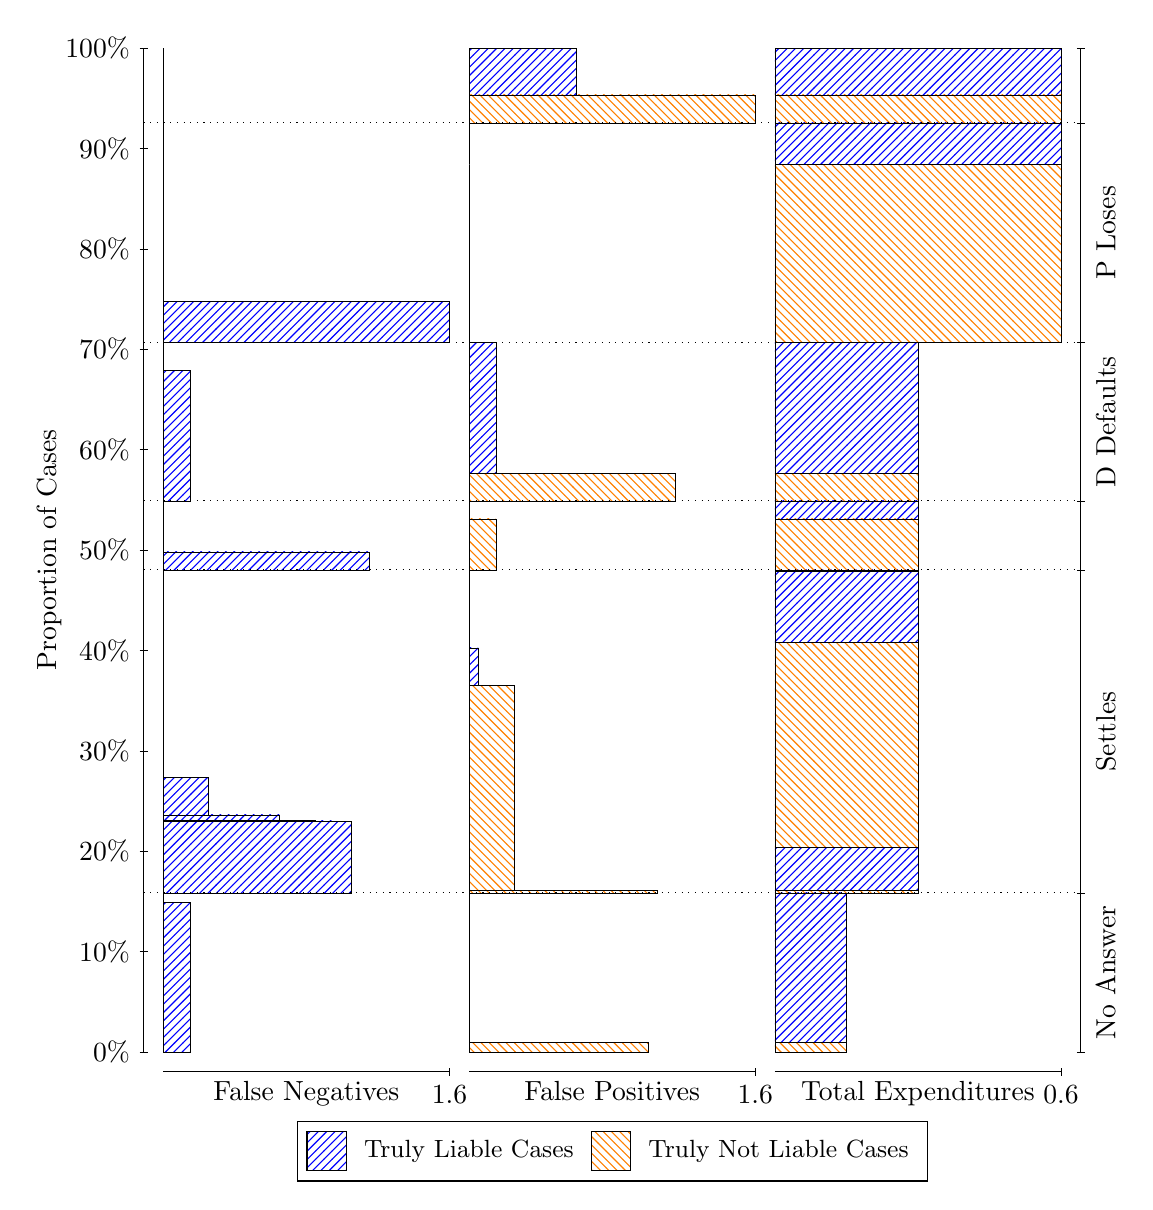
\begin{tikzpicture}
\draw[black, very thin] (1.5,1.75) -- (1.5,14.5);
\node[rotate=90, anchor=center] at (0.3, 8.125) {Proportion of Cases};
\draw[black, very thin] (1.45,1.75) -- (1.55,1.75);
\node[anchor=east] at (1.45, 1.75) {0\%};
\draw[black, very thin] (1.45,3.025) -- (1.55,3.025);
\node[anchor=east] at (1.45, 3.025) {10\%};
\draw[black, very thin] (1.45,4.3) -- (1.55,4.3);
\node[anchor=east] at (1.45, 4.3) {20\%};
\draw[black, very thin] (1.45,5.575) -- (1.55,5.575);
\node[anchor=east] at (1.45, 5.575) {30\%};
\draw[black, very thin] (1.45,6.85) -- (1.55,6.85);
\node[anchor=east] at (1.45, 6.85) {40\%};
\draw[black, very thin] (1.45,8.125) -- (1.55,8.125);
\node[anchor=east] at (1.45, 8.125) {50\%};
\draw[black, very thin] (1.45,9.4) -- (1.55,9.4);
\node[anchor=east] at (1.45, 9.4) {60\%};
\draw[black, very thin] (1.45,10.675) -- (1.55,10.675);
\node[anchor=east] at (1.45, 10.675) {70\%};
\draw[black, very thin] (1.45,11.95) -- (1.55,11.95);
\node[anchor=east] at (1.45, 11.95) {80\%};
\draw[black, very thin] (1.45,13.225) -- (1.55,13.225);
\node[anchor=east] at (1.45, 13.225) {90\%};
\draw[black, very thin] (1.45,14.5) -- (1.55,14.5);
\node[anchor=east] at (1.45, 14.5) {100\%};

\draw[black, very thin] (13.4,1.75) -- (13.4,14.5);
\draw[black, very thin] (13.35,1.75) -- (13.45,1.75);
\node[anchor=west] at (13.35, 1.75) {};
\draw[black, very thin] (13.35,3.7704) -- (13.45,3.7704);
\node[anchor=west] at (13.35, 3.7704) {};
\draw[black, very thin] (13.35,7.872) -- (13.45,7.872);
\node[anchor=west] at (13.35, 7.872) {};
\draw[black, very thin] (13.35,8.75) -- (13.45,8.75);
\node[anchor=west] at (13.35, 8.75) {};
\draw[black, very thin] (13.35,10.762) -- (13.45,10.762);
\node[anchor=west] at (13.35, 10.762) {};
\draw[black, very thin] (13.35,13.549) -- (13.45,13.549);
\node[anchor=west] at (13.35, 13.549) {};
\draw[black, very thin] (13.35,14.5) -- (13.45,14.5);
\node[anchor=west] at (13.35, 14.5) {};

\draw[black, very thin, pattern color=blue, pattern=north east lines] (1.75,1.75) rectangle (2.0906,3.6519);
\draw[black, very thin, pattern color=orange, pattern=north west lines] (1.75,3.6519) rectangle (1.75,3.7704);
\draw[black, very thin, pattern color=blue, pattern=north east lines] (1.75,3.7704) rectangle (4.1344,4.6816);
\draw[black, very thin, pattern color=blue, pattern=north east lines] (1.75,4.6816) rectangle (3.9073,4.6853);
\draw[black, very thin, pattern color=blue, pattern=north east lines] (1.75,4.6853) rectangle (3.6802,4.689);
\draw[black, very thin, pattern color=blue, pattern=north east lines] (1.75,4.689) rectangle (3.4531,4.6928);
\draw[black, very thin, pattern color=blue, pattern=north east lines] (1.75,4.6928) rectangle (3.226,4.7598);
\draw[black, very thin, pattern color=blue, pattern=north east lines] (1.75,4.7598) rectangle (2.3177,5.2346);
\draw[black, very thin, pattern color=orange, pattern=north west lines] (1.75,5.2346) rectangle (1.75,7.872);
\draw[black, very thin, pattern color=blue, pattern=north east lines] (1.75,7.872) rectangle (4.3615,8.1007);
\draw[black, very thin, pattern color=orange, pattern=north west lines] (1.75,8.1007) rectangle (1.75,8.75);
\draw[black, very thin, pattern color=blue, pattern=north east lines] (1.75,8.75) rectangle (2.0906,10.409);
\draw[black, very thin, pattern color=orange, pattern=north west lines] (1.75,10.409) rectangle (1.75,10.762);
\draw[black, very thin, pattern color=blue, pattern=north east lines] (1.75,10.762) rectangle (5.3833,11.287);
\draw[black, very thin, pattern color=orange, pattern=north west lines] (1.75,11.287) rectangle (1.75,13.549);
\draw[black, very thin, pattern color=orange, pattern=north west lines] (1.75,13.549) rectangle (1.75,13.904);
\draw[black, very thin, pattern color=blue, pattern=north east lines] (1.75,13.904) rectangle (1.75,14.5);
\draw[black, very thin, pattern color=orange, pattern=north west lines] (5.6333,1.75) rectangle (7.9042,1.8684);
\draw[black, very thin, pattern color=blue, pattern=north east lines] (5.6333,1.8684) rectangle (5.6333,3.7704);
\draw[black, very thin, pattern color=orange, pattern=north west lines] (5.6333,3.7704) rectangle (8.0177,3.7992);
\draw[black, very thin, pattern color=orange, pattern=north west lines] (5.6333,3.7992) rectangle (7.1094,3.8041);
\draw[black, very thin, pattern color=orange, pattern=north west lines] (5.6333,3.8041) rectangle (6.8823,3.8044);
\draw[black, very thin, pattern color=orange, pattern=north west lines] (5.6333,3.8044) rectangle (6.6552,3.8047);
\draw[black, very thin, pattern color=orange, pattern=north west lines] (5.6333,3.8047) rectangle (6.4281,3.8049);
\draw[black, very thin, pattern color=orange, pattern=north west lines] (5.6333,3.8049) rectangle (6.201,6.4077);
\draw[black, very thin, pattern color=blue, pattern=north east lines] (5.6333,6.4077) rectangle (5.7469,6.8825);
\draw[black, very thin, pattern color=blue, pattern=north east lines] (5.6333,6.8825) rectangle (5.6333,7.872);
\draw[black, very thin, pattern color=orange, pattern=north west lines] (5.6333,7.872) rectangle (5.974,8.5213);
\draw[black, very thin, pattern color=blue, pattern=north east lines] (5.6333,8.5213) rectangle (5.6333,8.75);
\draw[black, very thin, pattern color=orange, pattern=north west lines] (5.6333,8.75) rectangle (8.2448,9.1029);
\draw[black, very thin, pattern color=blue, pattern=north east lines] (5.6333,9.1029) rectangle (5.974,10.762);
\draw[black, very thin, pattern color=orange, pattern=north west lines] (5.6333,10.762) rectangle (5.6333,13.023);
\draw[black, very thin, pattern color=blue, pattern=north east lines] (5.6333,13.023) rectangle (5.6333,13.549);
\draw[black, very thin, pattern color=orange, pattern=north west lines] (5.6333,13.549) rectangle (9.2667,13.904);
\draw[black, very thin, pattern color=blue, pattern=north east lines] (5.6333,13.904) rectangle (6.9958,14.5);
\draw[black, very thin, pattern color=orange, pattern=north west lines] (9.5167,1.75) rectangle (10.425,1.8684);
\draw[black, very thin, pattern color=blue, pattern=north east lines] (9.5167,1.8684) rectangle (10.425,3.7704);
\draw[black, very thin, pattern color=orange, pattern=north west lines] (9.5167,3.7704) rectangle (11.333,3.8041);
\draw[black, very thin, pattern color=blue, pattern=north east lines] (9.5167,3.8041) rectangle (11.333,4.3459);
\draw[black, very thin, pattern color=orange, pattern=north west lines] (9.5167,4.3459) rectangle (11.333,6.9487);
\draw[black, very thin, pattern color=blue, pattern=north east lines] (9.5167,6.9487) rectangle (11.333,7.8599);
\draw[black, very thin, pattern color=orange, pattern=north west lines] (9.5167,7.8599) rectangle (11.333,7.8607);
\draw[black, very thin, pattern color=blue, pattern=north east lines] (9.5167,7.8607) rectangle (11.333,7.872);
\draw[black, very thin, pattern color=orange, pattern=north west lines] (9.5167,7.872) rectangle (11.333,8.5213);
\draw[black, very thin, pattern color=blue, pattern=north east lines] (9.5167,8.5213) rectangle (11.333,8.75);
\draw[black, very thin, pattern color=orange, pattern=north west lines] (9.5167,8.75) rectangle (11.333,9.1029);
\draw[black, very thin, pattern color=blue, pattern=north east lines] (9.5167,9.1029) rectangle (11.333,10.762);
\draw[black, very thin, pattern color=orange, pattern=north west lines] (9.5167,10.762) rectangle (13.15,13.023);
\draw[black, very thin, pattern color=blue, pattern=north east lines] (9.5167,13.023) rectangle (13.15,13.549);
\draw[black, very thin, pattern color=orange, pattern=north west lines] (9.5167,13.549) rectangle (13.15,13.904);
\draw[black, very thin, pattern color=blue, pattern=north east lines] (9.5167,13.904) rectangle (13.15,14.5);
\draw[black, dotted] (1.5,3.7704) -- (13.4,3.7704);
\draw[black, dotted] (1.5,7.872) -- (13.4,7.872);
\draw[black, dotted] (1.5,8.75) -- (13.4,8.75);
\draw[black, dotted] (1.5,10.762) -- (13.4,10.762);
\draw[black, dotted] (1.5,13.549) -- (13.4,13.549);
\draw[black, very thin] (1.75,1.5) -- (5.3833,1.5);
\node[anchor=north] at (3.5667, 1.5) {False Negatives};
\draw[black, very thin] (5.3833,1.45) -- (5.3833,1.55);
\node[anchor=north] at (5.3833, 1.45) {1.6};

\draw[black, very thin] (5.6333,1.5) -- (9.2667,1.5);
\node[anchor=north] at (7.45, 1.5) {False Positives};
\draw[black, very thin] (9.2667,1.45) -- (9.2667,1.55);
\node[anchor=north] at (9.2667, 1.45) {1.6};

\draw[black, very thin] (9.5167,1.5) -- (13.15,1.5);
\node[anchor=north] at (11.333, 1.5) {Total Expenditures};
\draw[black, very thin] (13.15,1.45) -- (13.15,1.55);
\node[anchor=north] at (13.15, 1.45) {0.6};

\node[black, centered, rotate=90] at (13.72, 2.7602) {No Answer};
\node[black, centered, rotate=90] at (13.72, 5.8212) {Settles};

\node[black, centered, rotate=90] at (13.72, 9.7558) {D Defaults};
\node[black, centered, rotate=90] at (13.72, 12.155) {P Loses};


\draw (7.449999999999999,1.5) node[draw=none] (baseCoordinate) {};
\begin{scope}[align=center]
        \matrix[scale=0.5, draw=black, below=0.5cm of baseCoordinate, nodes={draw}, column sep=0.1cm]{
            \node[rectangle, draw, minimum width=0.5cm, minimum height=0.5cm, pattern=north east lines, pattern color=blue] {}; &
            \node[draw=none, font=\small] (B) {Truly Liable Cases}; &
            \node[rectangle, draw, minimum width=0.5cm, minimum height=0.5cm, pattern=north west lines, pattern color=orange] {}; &
            \node[draw=none, font=\small] (B) {Truly Not Liable Cases}; \\
            };
\end{scope}

\end{tikzpicture}
\end{document}